\documentclass{standalone}
\usepackage{tikz}
\usepackage{ctex,siunitx}
\setCJKmainfont{Noto Serif CJK SC}
\usepackage{tkz-euclide}
\usepackage{amsmath}
\usetikzlibrary{patterns, calc,3d}
\usetikzlibrary {decorations.pathmorphing,decorations.pathreplacing,decorations.shapes}
\tikzset{label style/.append style={font=\small}}
% \newcommand\brickl{}
\begin{document}
\small
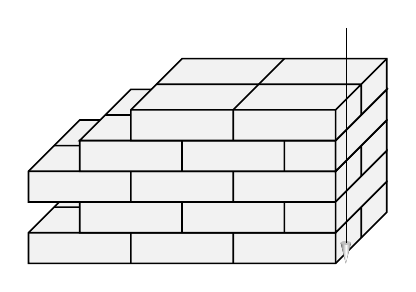
\begin{tikzpicture}[>=latex,scale=1.3,inner sep=1pt]
  \draw[semithick,fill=lightgray!20](-3,0)--(0,0)--(0.5,0.5)--(0.5,0.8)--(-2.5,0.8)--(-3,0.3)--cycle;
  \draw[semithick](-3,0.3)--(0,0.3)--(0.5,0.8)(0,0)--(0,0.3)(0.25,0.25)--(0.25,0.55)--(-2.75,0.55);
  \draw[semithick,fill=lightgray!20](-3,0.6)--(0,0.6)--(0.5,1.1)--(0.5,1.4)--(-2.5,1.4)--(-3,0.9)--cycle;
  \draw[semithick](-3,0.9)--(0,0.9)--(0.5,1.4)(0,0.6)--(0,0.9)(0.25,0.85)--(0.25,1.15)--(-2.75,1.15);
  \draw[semithick,fill=lightgray!20](-2.5,0.3)rectangle(0,0.6)(-2.5,0.9)rectangle(0,1.2)(0,0.3)--(0.5,0.8)--(0.5,1.1)--(0,0.6);
  \draw[semithick,fill=lightgray!20](-2.5,1.2)--(0,1.2)--(0.5,1.7)--(-2,1.7)--cycle(0,0.9)--(0.5,1.4)--(0.5,1.7)--(0,1.2)--cycle;
  \draw[semithick](0.25,1.45)--(-2.25,1.45);
  \draw[semithick,fill=lightgray!20](-2,1.2)--(0,1.2)--(0.5,1.7)--(0.5,2.0)--(-1.5,2.0)--(-2,1.5)--cycle;
  \draw[semithick](-2,1.5)--(0,1.5)--(0.5,2.0)(0,1.2)--(0,1.5)(0.25,1.45)--(0.25,1.75)--(-1.75,1.75);
  \draw[semithick](-1.5,0.3)--(-1.5,0.6)(-1.5,0.9)--(-1.5,1.2)(-0.5,0.3)--(-0.5,0.6)(-0.5,0.9)--(-0.5,1.2)(-2,0)--(-2,0.3)(-2,0.6)--(-2,0.9)(-1,0)--(-1,0.3)(-1,0.6)--(-1,0.9)(-1,1.2)--(-1,1.5)--(-0.5,2);
  \fill[left color=gray,right color=gray,middle color=white](0.1,0)--(0.05,0.2)--(0.15,0.2)--cycle;
  \fill[lightgray](0.1,0.2)ellipse(0.05 and 0.02);
  \draw[very thin](0.1,2.3)--(0.1,0.2);
\end{tikzpicture}
\end{document}